\documentclass[12pt,compress,aspectratio=169]{beamer}
\usetheme{metropolis}
\setbeamersize{text margin left=.5cm,text margin right=.5cm}
\usepackage[lf]{carlito}
\usepackage{siunitx}
\usepackage{tikz}
\usepackage{mathpazo}
\usepackage{bm}
\usepackage{mathtools}
\usepackage[ISO]{diffcoeff}
\diffdef{}{ op-symbol=\mathsf{d} }
\usepackage{xcolor,colortbl}

\setmonofont{Ubuntu Mono}
\setlength{\parskip}{0pt}
\renewcommand{\baselinestretch}{1}

\sisetup{
  inter-unit-product=\cdot,
  per-mode=symbol
}

\tikzset{
  >=latex
}

%\newcommand{\iii}{\hat{\bm\imath}}
%\newcommand{\jjj}{\hat{\bm\jmath}}
%\newcommand{\kkk}{\hat{\bm k}}


\usetikzlibrary{decorations.pathmorphing,patterns}

\title{Class 11: Universal Gravitation}
\subtitle{AP Physics C}
\author[TML]{Dr.\ Timothy Leung}
\institute{Olympiads School}
\date{Updated: Summer 2022}

\newcommand{\pic}[2]{
  \includegraphics[width=#1\textwidth]{#2}
}
\newcommand{\eq}[2]{
  \vspace{#1}{\Large
    \begin{displaymath}
      #2
    \end{displaymath}
  }
}
%\newcommand{\iii}{\ensuremath\hat{\bm{\imath}}}
%\newcommand{\jjj}{\ensuremath\hat{\bm{\jmath}}}
%\newcommand{\kkk}{\ensuremath\hat{\bm{k}}}
\newcommand{\iii}{\ensuremath\hat\imath}
\newcommand{\jjj}{\ensuremath\hat\jmath}
\newcommand{\kkk}{\ensuremath\hat k}



\begin{document}

\begin{frame}
  \maketitle
\end{frame}


\section{Gravitational Force}

\begin{frame}{Law of Universal Gravitation}
  \begin{center}
    \begin{tikzpicture}[scale=.65]
      \draw[vectors,red] (0,0)--(2,0) node[right]{$\vec F_{21}$};
      \draw[vectors,blue] (8,0)--(6,0) node[left]{$\vec F_{12}$};
      \shade[ball color=red] circle (.7) node[white]{$m_1$};
      \shade[ball color=blue] (8,0) circle (1)  node[white]{$m_2$};
      \draw[dashed] (0,0)--(0,-1.5);
      \draw[dashed] (8,0)--(8,-1.5);
      \draw[axes] (0,-1.3)--(8,-1.3) node[midway,below]{$\vec r_{12}$};
    \end{tikzpicture}
  \end{center}

  In classical mechanics, \textbf{gravity} is a mutually attractive force
  between massive objects, given by the \textbf{law of universal gravitation}:

  \eq{-.1in}{
    \boxed{
      \vec F_{12}=-G\frac{m_1m_2}{r_{12}^2}\hat r_{12}}
  }

  where $G=\SI{6.674e-11}{\newton.\metre\squared\per\kilo\gram\squared}$ is the
  \textbf{universal gravitational constant}, $r=|\vec r_{12}|$ is the distance
  between the centres of the masses, and $\hat r_{12}=\vec r_{12}/|\vec r_{12}|$
  is the unit vector pointing in the direction from $m_1$ to $m_2$.
\end{frame}



\begin{frame}{Law of Universal Gravitation}
  \begin{center}
    \begin{tikzpicture}[scale=.65]
      \draw[vectors,red] (0,0)--(2,0) node[right]{$\vec F_{21}$};
      \draw[vectors,blue] (8,0)--(6,0) node[left]{$\vec F_{12}$};
      \shade[ball color=red] circle (.7) node[white]{$m_1$};
      \shade[ball color=blue](8,0) circle (1)  node[white]{$m_2$};
      \draw[dashed] (0,0)--(0,-1.5);
      \draw[dashed] (8,0)--(8,-1.5);
      \draw[axes] (0,-1.3)--(8,-1.3) node[midway,below]{$\vec r_{12}$};
    \end{tikzpicture}
  \end{center}
  \begin{itemize}
  \item Third law of motion: If $m_1$ exerts a gravitational force $\vec F_{12}$
    on $m_2$, then $m_2$ likewise also exerts a reaction force of
    $\vec F_{21}=-\vec F_{12}$ on $m_1$. The two forces are equal in magnitude
    and opposite in direction
  \item $m_1$ and $m_2$ are \emph{point masses} that do not occupy any space
  \item The (more familiar) scalar form is often used as well:

    \eq{-.1in}{
      \boxed{F_g=G\frac{m_1m_2}{r^2}}
    }
  \end{itemize}
\end{frame}



\begin{frame}{More Than One Mass}
  \begin{columns}
    \column{.37\textwidth}
    \begin{tikzpicture}[scale=.4]
      \shade[ball color=red] circle (.7) node[white]{$M$};

      \draw[vectors,blue,rotate=45] (.7,0)--(2.5,0) node[right]{$\vec F_1$};
      \shade[ball color=blue] (5,5) circle (.8) node[white]{$m_1$};

      \draw[vectors,green,rotate=-45] (-.7,0)--(-2,0) node[left]{$\vec F_2$};
      \shade[ball color=green] (-5,5) circle (.6) node[white]{$m_2$};

      \draw[vectors,violet,rotate=45](-.7,0)--(-3.5,0) node[left]{$\vec F_3$};
      \shade[ball color=violet] (-5,-5) circle (1.2) node[white]{$m_3$};

      \draw[vectors,magenta,rotate=-45](.7,0)--(2.7,0) node[right]{$\vec F_4$};
      \shade[ball color=magenta] (5,-5) circle (.8) node[white]{$m_4$};

      %\draw[vectors] (.7,0)--(3.5,0) node[left]{$\vec F$};
    \end{tikzpicture}

    \column{.63\textwidth}
    For a mass that is subjected to the influence of multiple discrete point
    masses $m_i$, the total gravitational force that $M$ experiences is the
    vector sum of all the forces $\vec F_i$:
    
    \eq{-.1in}{
      \boxed{
        \vec F=\sum_i\vec F_i
        =GM\left(\sum_{i=1}^N\frac{m_i}{r_i^2}\hat r_i\right)
      }
    }
  \end{columns}
\end{frame}



\begin{frame}{Continuous Distribution of Mass}
  At the limit $N\rightarrow\infty$, the summation becomes an integral, and can
  now be used to describe the gravitational force from objects with
  \emph{spatial extend} i.e.\ masses that take up space (e.g.\ a continuous
  distribution of mass):

  \eq{-.1in}{
    \boxed{\vec F=\int\dl\vec F=GM\int\frac{\dl m}{r^2}\hat r
    }
  }

  Objects that are symmetrically spherical (e.g.\ planets are stars in our
  solar system) can be treated as point masses, and integration can be avoided.
  However, this is not always the case.
\end{frame}



\section{Gravitational Field}

\begin{frame}{Gravitational Field}
  We generally describe the gravitational force (weight) as:
  
  \eq{-.1in}{
    \boxed{\vec F_g=m\vec g}
  }

  To find $\vec g$, we group the variables in the law of universal gravitation:
    
  \eq{-.1in}{
    \vec F_g
    =\underbrace{\left[-\frac{Gm_1}{r^2}\hat r\right]}_{=\vec g}m_2
    =m_2\vec g
  }

  The vector field function $\vec g$ is known as the \textbf{acceleration due
    to gravity}, and \textbf{gravitational field}.
\end{frame}



\begin{frame}{Gravitational Field}
  On/near the surface of Earth, we can use

  \vspace{-.3in}{\large
    \begin{align*}
      m_1&=m_E=\SI{5.972e24}{\kilo\gram}\\
      r&=r_E=\SI{6.371e6}\metre
    \end{align*}
  }
  
  to obtain the commonly-known value of

  \vspace{-.3in}{\large
    \begin{align*}
      g &\approx\SI{9.81}{\metre\per\second\squared}\\
      g &\approx\SI{9.81}{\newton\per\kilo\gram}
    \end{align*}
  }

  both units are equivalent
\end{frame}



\begin{frame}{Gravitational Field}
  The \textbf{gravitational field} $\vec g$ generated by point mass $m$
  shows how it influences the gravitational forces on other masses:

  \eq{-.1in}{
    \boxed{g(m,\vec r)=-\frac{Gm}{r^2}\hat r}
  }
  \begin{center}
    \begin{tabular}{l|c|c}
      \rowcolor{pink}
      \textbf{Quantity} & \textbf{Symbol} & \textbf{SI Unit} \\ \hline
      Gravitational field       & $\vec g$ & \si{\newton\per\kilo\gram}\\
      Universal gravitational constant
      & $G$ & \si{\newton\metre\squared\per\kilo\gram\squared} \\
      Source mass               & $m$ & \si{\kilo\gram} \\
      Distance from source mass & $r$ & \si\metre \\
      Outward radial unit vector from source & $\hat r$ & N/A
    \end{tabular}
  \end{center}
  The negative sign indicates that \emph{direction} of the gravitational field
  is towards $m$.
\end{frame}



\begin{frame}{More Than One Mass}
  When multiple point masses are present, the total gravitational field at any
  position $\vec r$ is the vector sum of all the fields $\vec g_i$:
    
  \eq{-.1in}{
    \boxed{\vec g
      =\sum_i\vec g_i
      =G\left(\sum_{i=1}^N\frac{m_i}{r_i^2}\hat r_i\right)
    }
  }

  At the limit $N\rightarrow\infty$, the summation becomes an integral, and can
  now be used to describe the gravitational field generated by objects with
  \emph{spatial extend}:

  \eq{-.1in}{
    \boxed{\vec g
      =\int\dl\vec g
      =G\int\frac{\dl m}{r^2}\hat r
    }
  }
  
  This integral may be difficult to compute, if the geometry is complicated.
\end{frame}




\begin{frame}{Relating Gravitational Field \& Gravitational Force}
  When a mass $m$ is placed inside a gravitational field $\vec g$, it
  experiences a gravitational force given by the familiar equation:
  %$\vec g$ itself doesn't \emph{do} anything unless/until another mass $m$
  %enters the field. Then, $m$ experiences a gravitational force $\vec F_g$
  %proportional to $m$ and $\vec g$, regardless of how the field is created:

  \eq{-.1in}{
    \boxed{\vec F_g=m\vec g}
  }
%  \begin{center}
%    \begin{tabular}{l|c|c}
%      \rowcolor{pink}
%      \textbf{Quantity} & \textbf{Symbol} & \textbf{SI Unit} \\ \hline
%      Gravitational force on a mass & $\vec F_g$ & \si\newton \\
%      Mass inside the gravitational field & $m$ & \si{\kilo\gram}\\
%      Gravitational field & $\vec g$   & \si{\newton\per\kilogram}
%    \end{tabular}
%  \end{center}
  Note: A mass is not affected by the gravitational field that itself
  generates.
\end{frame}



\begin{frame}
  \centering
  \begin{tikzpicture}
    \draw[blue!70!black,mass] circle (.3) node[midway]{$M$};
    \foreach \theta in {0,45,...,359}
    \draw[vectors,blue!70!black,rotate=\theta] (2,0)--+(-1,0);
    \foreach \theta in {0,30,...,359}
    \draw[vectors,blue!70!black,rotate=\theta] (3,0)--+(-.4,0);
    \node[right,blue!70!black] at (2,0) {$\vec g$};
    \node[
      text width=140,
      draw=blue!70!black,
      fill=blue!5,
      text=blue!70!black] at (5.7,0) {$M$ generates a gravitational field
      that extends from the mass itself over the entire space, with a magnitude
      of

      \vspace{-.07in}
      \begin{displaymath}
        g=\frac{GM}{r^2}
      \end{displaymath}
      $\vec g$ points \emph{towards} the mass that generated it.
      \par
    };
    \uncover<2->{
      \begin{scope}[orange,rotate=20]
        \draw[vectors] (-3.5,0)--+(1.2,0) node[right=0]{$\vec F_g$};
        \draw[thick,fill=orange!5] (-3.5,0) circle (.18) node{$m$};
      \end{scope}
      \node[
        text width=220,
        draw=orange,
        fill=orange!5,
        text=orange] at (-2.7,-3.6){Mass $m$ is inside the gravitational field
        generated by {\color{blue!70!black}$M$}, therefore it experiences a
        gravitational force of
        
        \vspace{-.08in}
        \begin{displaymath}
          \vec F_g=m{\color{blue!70!black} \vec g}
        \end{displaymath}
        The gravitational force is in the same direction as
        {\color{blue!70!black}$\vec g$}\par
      };
    }
    
    \node[text width=160,text=blue!70!black] at (5.3,-3) {The
      gravitational field generated by $M$ does not do anything until there
      is another mass inside the field.\par
    };
  \end{tikzpicture}
\end{frame}



\begin{frame}{What If You Are Inside Another Mass?}
  \begin{columns}
    \column{.3\textwidth}
    \begin{tikzpicture}[scale=.45]
      \draw[thick,fill=gray] circle(5) node[above]{$m_1$};
      \draw[thick,fill=black!2] circle(4.9);
      \draw[axes,rotate=30] (0,0)--(4.9,0) node[midway,below]{$R$};
      \draw[mass] (1,-1) circle(.2) node[below]{$m_2$};
    \end{tikzpicture}

    \column{.7\textwidth}
    Newton used the \textbf{shell theorem} to show that if a mass $m_2$ is
    \emph{inside} a spherical shell of mass $m_1$, the gravitational force that
    it experiences is \emph{zero}.
      
    \eq{-.1in}{
      \boxed{
        \vec F_g=
        \begin{cases}
          \vec 0 & \text{if}\;\;r<R\\
          -Gm_1m_2/r^2\hat r & \text{otherwise}
        \end{cases}
      }
    }
      
    It also means that gravitational field is also \emph{zero} inside the shell
  \end{columns}
\end{frame}



\begin{frame}{What If You Are Inside Another Mass?}{A Spherical Shell}
  \begin{columns}
    \column{.3\textwidth}
    \begin{tikzpicture}[scale=.45]
      \draw[thick,fill=gray] circle (5);% node[above]{$m_1$};
      \draw[thick,fill=black!2] circle (4.9);% node[above]{$m_1$};
      \draw[axes,rotate=30] (0,0)--(4.9,0) node[midway,below]{$R$};
      \draw[mass] (1,-1) circle (.2) node[below]{$m_2$};
    \end{tikzpicture}

    \column{.7\textwidth}
    That $\vec g_\text{inside}=\vec 0$ can be calculated by:
    \begin{itemize}
    \item Integrating the fields created by infinitesimal mass elements $\dl m$
      at any point inside the shell, or
    \item Using \textbf{Gauss's law} for gravity, similar to finding the
      electric field inside a charged conducting sphere:
      
      \eq{-.1in}{
        \oint\vec g\cdot\dl\vec A=-4\pi GM_\text{encl}
      }

      \vspace{-.07in}This method will be addressed in detail for
      \emph{electric} field in the E\&M portion of this course
    \end{itemize}
  \end{columns}
\end{frame}



\begin{frame}{Gravitational Field Inside a Spherical Shell}
  The gravitational field strength inside spherical shell is:
  \begin{center}
    \begin{tikzpicture}
      \draw[axes] (0,0)--(0,3) node[right]{$|\vec g|$};
      \draw[axes] (0,0)--(5.5,0) node[right]{$r$};
      \draw[thick,dashed] (1,0)--(1,2) node[pos=0,below]{$R$}--(0,2)
      node[left]{$\dfrac{GM}{R^2}$};
      \draw[functions,samples=15,smooth,domain=1:5] plot(\x,{2/\x});
      \draw[functions] (0,0)--(1,0);
      \draw[functions,fill=black!2] (1,0) circle (.06);
      \fill[red!80!black] (1,2) circle (.06);
    \end{tikzpicture}
  \end{center}
\end{frame}



\begin{frame}{What If You Are Inside Another Mass?}%{Uniform Mass of Radius $R$}
  \begin{columns}
    \column{.35\textwidth}

    \begin{tikzpicture}[scale=.45]
      \draw[thick,fill=gray!50] circle(5);
      \draw[thick,fill=gray!10] (-.2,5) rectangle(.2,-5);
      \draw[mass] (0,1) circle(.15) node[right,black]{$m$};
    \end{tikzpicture}

    \column{.65\textwidth}
    Suppose you could drill a hole through the Earth and then jump into it. How
    long would it take you to emerge on the other side of the Earth?

    \vspace{.2in}To calculate this, we need to know how the gravitational force
    changes as you fall through Earth.
  \end{columns}
\end{frame}




\begin{frame}{Falling Towards the Centre of Earth}
  \begin{columns}
    \column{.3\textwidth}
    \pic1{eartholeg}

    \column{.7\textwidth}
    As you fall through Earth, we can separate the part of Earth that is
    ``above'' you, and the part that is ``below'' you
    \begin{itemize}
    \item The part that is ``above'' you is like the spherical shell, and does
      not contribute to the gravitational field, and therefore does not exert
      any force
    \item The part that is ``below'' you gets smaller as you fall towards the
      centre
    \end{itemize}
  \end{columns}
\end{frame}



\begin{frame}{Falling Towards the Centre of Earth}
  Assuming that Earth's density is uniform, and neglecting air resistance and
  other factors, the value of $g$ as the person falls through Earth ($r<R$) is
  given by finding how much mass is still ``below'' the person, $M(r)$:

  \eq{-.1in}{
    g(r)=\frac{GM(r)}{r^2}\quad\quad M(r)=\frac43\rho\pi r^3\quad\quad
    \rho=\frac{3M_E}{4\pi r_E^3}
  }

  where $M_E$ is the mass of Earth, $r_E$ is the radius of Earth, $\rho$ is the
  (constant) density, and $r$ is the distance from Earth's centre. Then $M(r)$
  is the amount of mass ``below'' the person as he/she falls towards the centre.
\end{frame}



\begin{frame}{Falling Towards the Centre of Earth}
  \begin{columns}
    \column{.3\textwidth}
    \pic1{eartholeg}

    \column{.7\textwidth}
    The gravitational field strength inside this hypothetical Earth is a
    linear function of distance $r$ from the centre:

    \eq{-.1in}{
      g(r)=\frac{GM_E r}{r_E^3}=\left(\frac r{r_E}\right)g_0
    }
    
    where $g_0=\SI{9.81}{\newton\per\kilogram}$ is the field strength at the
    surface. At the centre ($r=0$), $g=0$. The gravitational force is:
    
    \eq{-.1in}{
      F_g(r)=-\underbrace{\left[\frac{mg_0}{r_E}\right]}_k r
    }
  \end{columns}
\end{frame}



\begin{frame}{Gravitational Field Strength Inside a Uniform Sphere}
  The gravitational field strength inside a uniform sphere is:
  \begin{center}
    \begin{tikzpicture}
      \draw[axes] (0,0)--(0,3) node[right]{$|\vec g|$};
      \draw[axes] (0,0)--(5.5,0) node[right]{$r$};
      \draw[thick,dashed] (1,0)--(1,2) node[pos=0,below]{$R$}--(0,2)
      node[left]{$\dfrac{GM}{R^2}$};
      \draw[functions,domain=1:5] plot(\x,{2/\x});
      \draw[functions] (0,0)--(1,2);
    \end{tikzpicture}
  \end{center}
\end{frame}



\begin{frame}{Falling Towards the Centre of Earth}
  \begin{columns}
    \column{.25\textwidth}
    \pic1{eartholsat}

    \column{.75\textwidth}
    The gravitational force has the same form as Hooke's law: it is
    proportional to displacement from the centre, but in the opposite
    direction:

    \eq{-.2in}{
      F_g(r)=-kr
    }
    
    \vspace{-.1in}The motion is a simple harmonic motion. The traveler will
    oscillate through Earth with a period of:

    \eq{-.1in}{
      T=2\pi\sqrt{\frac mk}=2\pi\sqrt{\frac{r_E}{g_0}}
    }

    For Earth, $T=\SI{5068}\second$. The traveler would pop up on the opposite
    side every \SI{42}{min}.
  \end{columns}
\end{frame}




\begin{frame}{Falling Towards the Centre of Earth}
  \begin{columns}
    \column{.25\textwidth}
    \pic1{eartholsat}

    \column{.75\textwidth}
    Since simple harmonic motion is a projection of a uniform circular motion,
    if a satellite is in a circular orbit just above the surface, and passes
    overhead just above the traveler as he/she popped up out of the hole. The
    period of such an orbit would be the same as oscillating traveler.
  \end{columns}
\end{frame}



\begin{frame}{Gravitational Field Lines}
  \begin{center}
    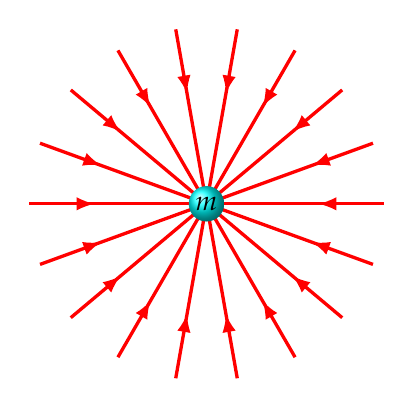
\begin{tikzpicture}[scale=1.5]
      \foreach \x in {0,20,...,359}{
        \begin{scope}[red,very thick,rotate=\x]
          \draw (0,0)--(1,0);
          \draw[<-](.95,0)--(1.5,0);
        \end{scope}
      }
      \shade[ball color=cyan] circle(.15) node{$m$};
    \end{tikzpicture}
  \end{center}
  \begin{itemize}
  \item The direction of $\vec g$ is towards the centre of the object that
    created it
  \item Field lines do not tell the intensity (i.e.\ magnitude) of $\vec g$,
    only the direction
  \end{itemize}
\end{frame}



\begin{frame}{Gravitational Field Lines}
  When there are multiple masses, the total gravitational field (dotted line)
  is the vector sum of all the individual fields.
  \begin{center}
    \pic{.4}{grav-fields}
  \end{center}
  The solid lines are called \textbf{equipotential lines}, where the potential
  energy is constant. Equipotential lines are perpendicular to
  gravitational field lines.
\end{frame}



\section{Gravitational Potential Energy}

\begin{frame}{Gravitational Potential Energy}
  \textbf{Gravitational potential energy} is found by integrating the work
  done by the gravitational force:

  \vspace{-.2in}{\large
    \begin{align*}
      W_g &=\int \vec F_g\cdot\dl\vec r
      =-\int_{r_1}^{r_2}\frac{Gm_1m_2}{r^2}\hat r\cdot\dl\vec r
      =-\int_{r_1}^{r_2}\frac{Gm_1m_2}{r^2}dr\\&=\frac{Gm_1m_2} r\Big|^{r_2}_{r_1}
      =-\Delta U_g
    \end{align*}
  }

  where the \textbf{gravitational potential energy} is defined as
  
  \eq{-.1in}{
    \boxed{U_g=-\frac{Gm_1m_2}r}
  }
  \begin{itemize}
  \item $U_g$ is the work required to move two objects from $r$ to $\infty$
  \item $U_g=0$ at $r=\infty$ and \emph{decrease} as $r$ decreases
  \end{itemize}
\end{frame}



\begin{frame}{Gravitational Potential Energy}
  As we have seen before, the work done by gravity is related to the
  gravitational potential energy by:
  
  \eq{-.1in}{
    \boxed{
      W_g=-\Delta U_g
    }
  }

  \fcolorbox{black}{yellow!10}{
    \begin{minipage}{.98\textwidth}
      \begin{itemize}
      \item $(+)$ work by gravity decreases gravitational potential energy
      \item $(-)$ work by gravity increases gravitational potential energy
      \item $W_g$ depends on $r_0$ and $r_1$, but not \emph{how}
        it goes from $r_0\rightarrow r_1$ (path independence)
      \item Only work done by gravity can affect gravitational potential energy
      \end{itemize}
    \end{minipage}
  }
\end{frame}



\begin{frame}{Relating Gravitational Potential Energy to Force}
  The fundamental theorem of calculus shows that gravitational force
  ($\vec F_g$) is the negative gradient of the gravitational potential energy
  ($U_g$):
  
  \eq{-.1in}{
    \vec F_g = -\nabla U_g = -\diffp{U_g}r\hat r
  }

  The direction of $\vec F_g$ always points from high to low potential energy
  \begin{itemize}
  \item A free-falling object is always decreasing in $U_g$
  \item ``Steepest descent'': the direction of $\vec F_g$ is the shortest path
    to decrease $U_g$ 
  \item Objects traveling perpendicular to $\vec F_g$ has constant $U_g$
  \end{itemize}
\end{frame}



\begin{frame}{Relating $U_g$, $\vec F_g$ and $\vec g$}
  Knowing that $\vec F_g$ and $\vec g$ only differ by a constant (mass $m$), we
  can also relate gravitational field to potential energy by the gradient
  operator:

  \eq{-.1in}{
    \vec g=-\nabla V_g=-\diffp{V_g}r\hat r
    \quad\text{where}\quad
    V_g=\frac{U_g}m
  }

  We already know that the direction of $\vec g$ is the same as $\vec F_g$,
  i.e.
  \begin{itemize}
  \item The direction of $\vec g$ is the shortest path to decrease $U_g$ 
  \item Objects traveling perpendicular to $\vec g$ has constant $U_g$
  \item $V_g$ is called the \textbf{gravitational potential} but
    it is rarely used
  \end{itemize}
\end{frame}
\end{document}
